\section{System, Assumptions and Problem Formulation}
\label{sec:problemformulation}

% Background and problem model
\subsection{System and Assumptions}
\label{subsec:model}

% Background
% Multiband variation
Wireless propagation refers to the signal loss characteristics when wireless signals 
are transmitted through the wireless medium. The strength of the received signal depends on 
both the line-of-sight path (or lack thereof) and multiple other paths that result from reflection, 
diffraction, and scattering from obstacles~\cite{andersen1995propagation}. The widely-used Friis
equation characterizes the received signal power $P_r$ in terms of transmit power $P_t$, transmitter 
gain $G_t$, receiver gain $G_r$, wavelength $\lambda$ of the carrier frequency, distance $R$ from 
transmitter to receiver, and path loss exponent $n$ according to~\cite{friis}:
\begin{equation}
\label{eq:friis}
P_r=P_t+G_t+G_r+10n \log_{10}\left( \frac{\lambda}{4\pi R}\right)
\end{equation}
Here, $n$ varies according to the aforementioned environmental 
factors with a value ranging from two to five in typical outdoor 
settings~\cite{rappaport}.
% Tell the propagation of white space is much larger than wifi
Thus, the channels of white space bands propagates further than the channels of the WiFi bands in 
free space under the same RSSI threshold, transceiver settings~\ref{eq:friis}. 
% White spcae is good out resource to improve the service of Wifi cell
The propagation range of white space channels could be many times of WiFi channels, for instance, 
450 MHz channels has more than 12 times propagation range as 5 GHz channels. The larger propagation 
of white space channels make it possible to assist a WiFi mesh with few white space channels. 
% Power saving


\begin{figure}
\vspace{-0.0in}
\centering
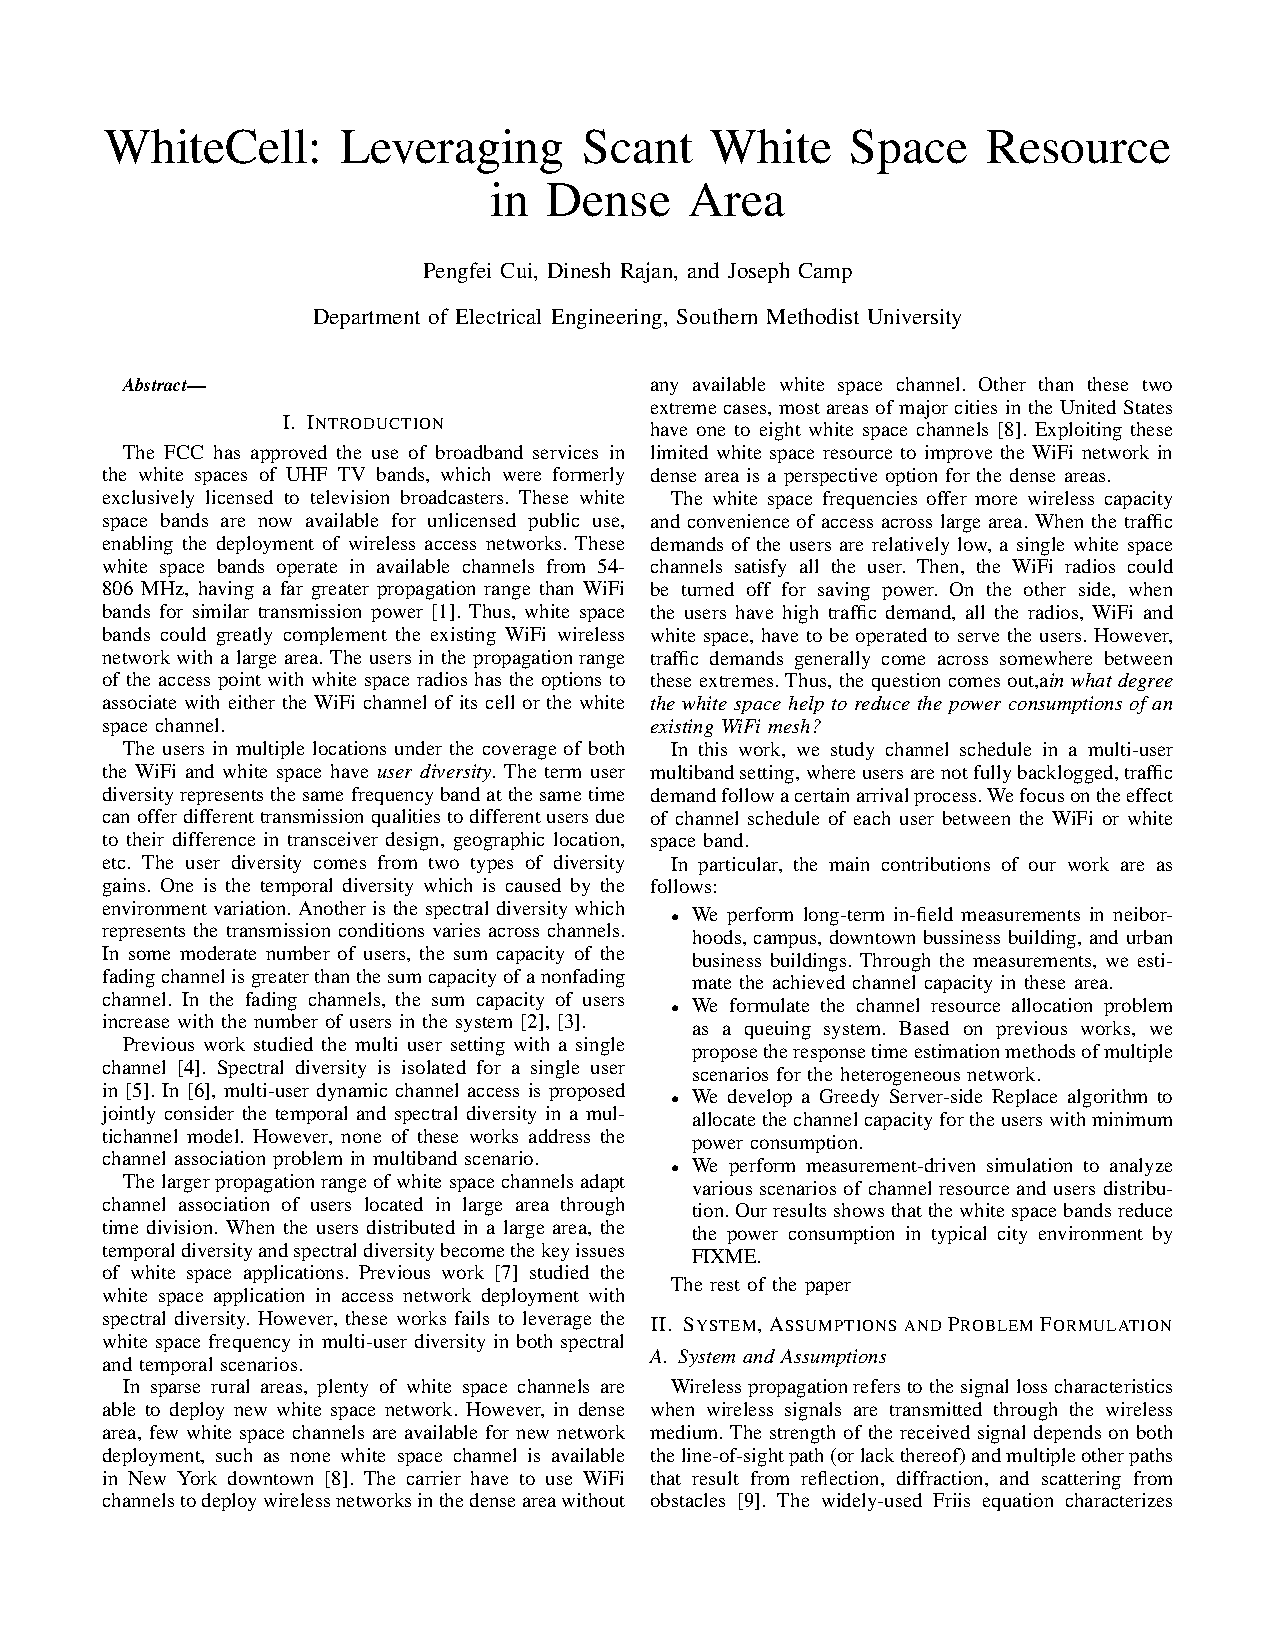
\includegraphics[width=74mm]{figures/whitecell}
\vspace{-0.1in}
\caption{White Space Model in Dense Area}
\label{fig:systemmodel}
\vspace{-0.1in}
\end{figure}


% Give the model and assumption
% B channel; N user; M AP;
Given a WiFi mesh wireless system with $M$ access points and $N$ users as shown in Fig.~\ref{fig:systemmodel}. 
The users are scheduled with the access point on the single channel $f \in F_M$ located in its own mesh. 
We consider $F_w$ new white space radios is installed on one of the access points to assistant the existing WiFi 
network. The capacity of each radio $C$ is a equally restrict number of all the channels. 
Each radio has enough buffer store the traffic demand. 
The traffic is served in a FIFO system.
For each user, it 
has $1+F_w$ channels to be scheduled, the previous in-cell WiFi channel and the new white space channels. 
Instead of assuming the wireless are on-off~\cite{bodas2012low}, we apply our measurements to estimate the 
channel capacity. The capacity of the scheduled channels between the access points and users is noted as a 
matrix in Eq.~\ref{eq:usercapacity}
\begin{equation}
\label{eq:usercapacity}
H_{i,j}^f(t)= G(\zeta,t),i \in M, j\in N, f \in (F_M+F_w) 
\end{equation} 
$\zeta$ represents the in-field measured historical data and dynamic sensing information.
We use a context-aware method to estimate the $j$ user capacity $H_{i,j}^f(t)$ to an access point 
$i$ on channel $f$. 
We assume the users from the same mesh cell are in a single interference domain.
%These users share  a time division for the WiFi channel assigned for this cell. 
Considering the limited number of white space channels in dense area and the fact spatial reuse 
of white space will make the problem considerably more challenging, we will remains an interesting 
direction of future research. 
% Enough channel resource given
%We assume there are enough channel resource given for the system according to worst channel capacity 
%state $H_{i,j}^{f*}(t)$.


We assume the channel capacity is flat during a time slot. We also assume the switching time is negligible. 
The traffic demand arrive at a user as a Poisson process, with the vector noted as $\bm{D(t)} = [D_1(t),D_2(t),...D_N(t)]$ 
and the sum rate $D(t) = \sum\limits_{i=1}^N D_i(t)$.  The rate $D(t)$ is the aggregate rate of data 
generated from all users. 



% Buffer and tolerance time
In a time slot, we assume the unscheduled radios remain in sleep mode to save energy. 
Also we ignore the sleeping energy as well as the amount of energy spent on channel/radio 
switching. An operating radio will cost equal power during a time unit. 
Previous work~\cite{niida2010user} shows a user has a certain patience for waiting. 
The tolerance time varies across the traffic type, such as text information, 
voice information. 
To simply the problem, we assume an arbitrary average 
value for $W$ of the users in the area. 
The system apply a first-come-first-serve schedule. 


%The served traffic flow $\Gamma$ represents the traffic  
%delivered to the access points through the wireless channels.


%As discussed in ~\cite{niida2010user}, the tolerance 
%time of traffic varies from text information, voice information. To address the user tolerance time, we 
%have the waiting time constraint $\mu_j,j\in N$ based on the users traffic demand types.  
% Buffer assumptions
%Through this waiting time constraint, the waiting time of a user is limited in a certain time window, 
%which means the traffic of a user will be served during the tolerance time to satisfy the QoS requirements.
%We define the payoff function according to the waiting time of user's traffic and traffic types in Eq.\ref{eq:payoff}. 
%To address the user tolerance time, we build the payoff functions based on the users traffic demand and the buffered time of the 
%traffic demand to process the channel schedule. Through this payoff function, the waiting time of a user is limited in 
%a certain time window, which means a user will be served at least once to satisfy the QoS requirements.
%We define the payoff function according to the waiting time of user's traffic and traffic types in Eq.\ref{eq:payoff}. 
%
%% Payoff B, benefit
%\begin{equation}
%\label{eq:payoff}
%\xi=\sum \alpha^{t_d}\cdot T
%\end{equation}
%%$\alpha$ is a parameter represents the traffic types. 
%To represents the variation, we define the $\alpha \ge 1$ to represent the tolerance of traffic
%type to make an individual user stay in the tolerance time. 
%$t_d$ is the time the user has waited for the traffic in the queue. Through the definition, the traffic could be 
%scheduled according to the traffic type and the waiting time. 
%According the the payoff function, the expected benefit of a served beam schedule could be calculated through the BBS framework.
%With BBS, the time efficient for the system is increased and the satisfaction of users and power efficient.




\subsection{Problem Formulation}
\label{subsec:problem}


We formulate the system discussed in~\ref{subsec:model} as a discrete-time queuing system as shown in 
Fig.~\ref{fig:flowconfig}. The channels are represented as servers in the queuing system. Table.~\ref{tab:notation} 
summarizes the notation used in this work. The queuing system has $N$ queues and $F_M+F_w$ servers connecting 
by time-varying channels $H^*(N,F_M+F_w)$.


\begin{table}[htbp]
\begin{center}% used the environment to augment the vertical space
% between the caption and the table
\begin{tabular}{l l p{10cm} }
\toprule
$t$ & Time slot\\
$N$ & Set of users\\
$M$ & Set of WiFi cells\\
$H_{ij}^f$ & Measurement based Capacity between AP i and user j on channel f\\
$F_{m}$ & WiFi Channels in the cells\\
$F_{w}$ & Set of White Space Channels\\
$A(t)$ & User access channel schedule\\
$C$ & Clean Radio Capacity\\
$D$ & User Demand\\
$R$ & Operating Radio\\
$\zeta$ & In-Field Measurements\\
$W$ & User Tolerance time window \\
$\mu$ & Channel capacity assigned for a cell \\
$P_s$ & Standby Power Consumption \\
$P_t$ & Transmission Power Consumption \\
%$R_{i}$ & $\triangleq$ & Revenue at store $i$\\
%$i$ & $\triangleq$ & index value for store locations\\
%${T}_{c}$ & $\triangleq$ & A very long description of this specific variable and is needed in the research and looks good when wrapped and aligned to the left.\\
%$TC$ & $\triangleq$ & Total overall cost(\$)\\  
%\multicolumn{3}{c}{}\\
%\multicolumn{3}{c}{\underline{Decision Variables}}\\
%\multicolumn{3}{c}{}\\
%$y_f$ & $=$ & \(\left\{\begin{array}{rl}
%1,  & \text{if Supplier located at site $f$ is open} \\
%0,  & \text{otherwise} \end{array} \right.\)\\
\bottomrule
\end{tabular}
\end{center}
\caption{Table of Notations}
\label{tab:notation}
\vspace{-0.3in}
\end{table}





\begin{figure}
\vspace{-0.0in}
\centering
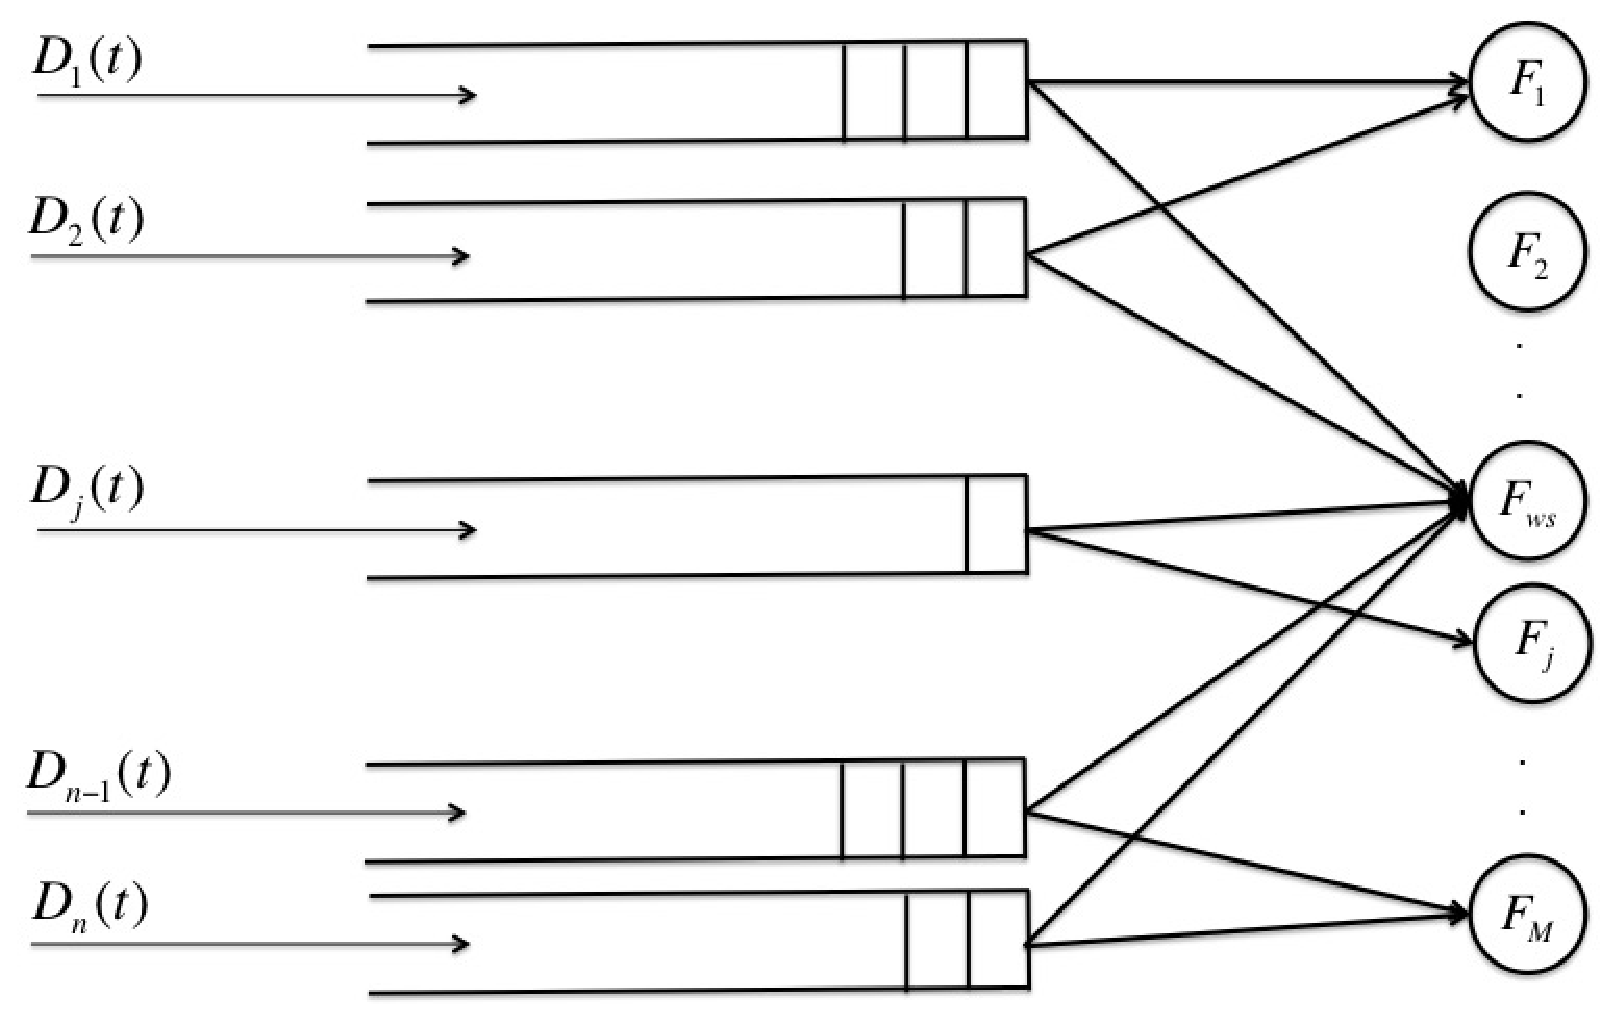
\includegraphics[width=84mm]{figures/flowconfig}
\vspace{-0.1in}
\caption{System Model}
\label{fig:flowconfig}
\vspace{-0.1in}
\end{figure}


In this system, during a time unit, the users need to schedule with their achieved channels. 
Let matrix \{$A_{i,j}(t),i\in (F_M+F_w), j\in N$\} denote a schedule meets the performance constraints 
will be discussed later.
%where $A_{i,j}^b = 1$ denotes user $j$ is scheduled with access point $i$ on channel $b$.
\begin{equation}
\label{eq:associate_def}
 A_{i,j}(t) = \left\{ 
	  \begin{array}{l l}
	    1   &  if\ D_{j\in N},\ is\ scheduled\ with\ \\
		& channel\ i \in (F_M+F_w) \\
		0 &  Otherwise
			    \end{array} \right.
\end{equation}

% System constraint, buffer, waiting time
%The traffic is a Poisson process, which means the users could store part of the traffic in the 
%buffer. Thus, the expected length of the queue should be less than the buffer as shown in Eq.~\ref{eq:bufferconstraint} 
%\begin{equation}
%\label{eq:bufferconstraint}
%%\sum\limits_{t^*}^{t^*+\mu_j}\gamma_j(t^*) \ge Q(t^*)+D(t^*), j\in N
%E[Q_j] \le B , j\in N
%\end{equation}
%$B$ is the buffer size of a user.

To satisfy the users, the system need to keep the expected waiting time of the system $w$ need to be less than the 
threshold $W$ as shown in Eq.~\ref{eq:timeconstraint}
\begin{equation}
\label{eq:timeconstraint}
E[w]\le W
\end{equation}


With the intuition, when the total traffic demand of the users in the system are small, one white space radio in 
white space could achieve the quality of service for the users. Thus all the WiFi radios could be turned down. 
However, as the traffic demand increase with the number of users or the demand per user, we need to increase the 
channel resource from the system to satisfy the user requirements. 
Another advantage scenario of white space channels are when some of the WiFi cells have more traffic demand, we can spend more 
white space channel capacity for these cells without building new infrastructure. 
Then the questions come as, how much power we could save through divide the white space capacity into the WiFi cells? 
And how much user traffic demand variation we could adapt in one or more cells in the system?





